% Drawing 144/07-1 -- folder 144, batch 07, archive page 125 (PDF page 126).
% Transcription: à droite, sous l'inscription $\mathcal{M}''^!_0$, un réseau en perspective (double pyramide) dont les sommets sont $\mathcal{M}^!_0$, $\underline{\mathcal{M}}^!$, $\underline{\mathcal{M}}$, $\underline{\mathcal{M}}'$, $\mathcal{M}'''$, $\underline{\mathcal{M}}''$, $\mathcal{M}'^!_0$, $\mathcal{M}'''^!_0$, $\mathcal{M}''^!_0$, $\mathcal{M}'^!$, $\mathcal{M}'''^!$, $\mathcal{M}''^!$, $\mathcal{M}^{!\circ}$, $\mathcal{M}^{\circ}$, $\underline{\mathcal{M}}^{!\circ}_0$ ; les arêtes portent les indices 2, 6, 12, et des arêtes pointillées verticales relient les sommets $'''$ aux sommets voisins. Dessous, au crayon, l'esquisse d'un cube $\mathcal{M}^!_0$, $\mathcal{M}^!$, $\mathcal{M}$, $\mathcal{M}^{!\circ}_0$, $\mathcal{M}^{!\circ}$ et d'autres polyèdres non étiquetés.
% Kind: three double pyramids of moduli spaces joined by coverings of degree 2 and 6. Method 2 (schematic redraw from the facsimile). Status: partial.
% Notes: Landscape sheet (page turned). Under the inscription M''^!_0, three double pyramids in perspective (one per level: _0 with !, with !, without !), corresponding vertices joined left to middle (degree 2) and middle to right (degree 6); edges inside each pyramid marked 2, verticals through the centre vertex (''') dotted. Vertex names placed as read; which of them carry an underline is partly uncertain. The pencil sketch of a cube and other polyhedra below (left half of the sheet) and the text under the figure are not drawn.
% Coordinates: 1 unit = 1 mm = 1/100 of the crop width (bbox in page fractions: [0.62, 0.13, 0.94, 0.33]).
% Redrawn by Claude (claude-opus-5-5), issue #73, 2026-11-07; not checked by a human; not compiled (no TeX in the session).
% Rights: reproduces part of the work -- behind RENDER_TRANSCRIPTS, never published by itself.
\documentclass[tikz,border=3pt]{standalone}
\usepackage{amsmath,amssymb}
\usetikzlibrary{patterns,arrows.meta}
\tikzset{pencil/.style={black!45}, struck/.style={black!35}, mark/.style={circle,draw,inner sep=1.3pt}, pt/.style={circle,fill,inner sep=0.9pt}, opt/.style={circle,draw,fill=white,inner sep=1.1pt}}
\begin{document}
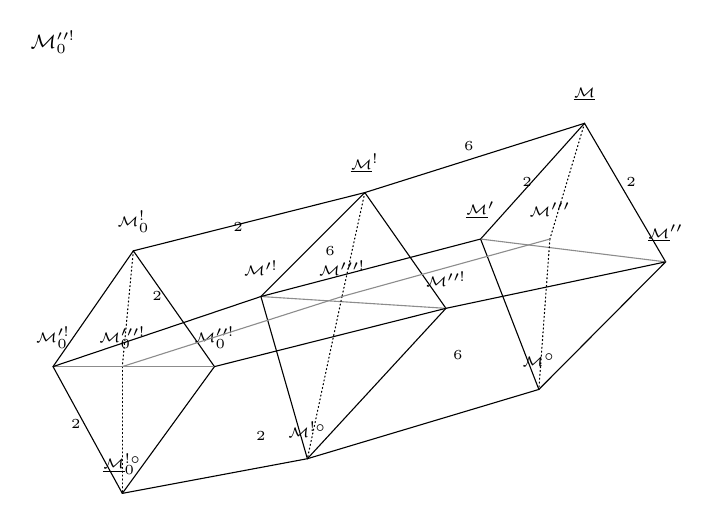
\begin{tikzpicture}[x=1mm,y=1mm,line cap=round,line join=round,font=\scriptsize]
\node[inner sep=1pt] at (11,-8.7) {\scriptsize $\mathcal M''^!_0$};
\draw (21.2,-35.2) -- (11,-49.9);
\draw (21.2,-35.2) -- (31.5,-49.9);
\draw (11,-49.9) -- (19.8,-66);
\draw (31.5,-49.9) -- (19.8,-66);
\draw[pencil] (11,-49.9) -- (31.5,-49.9);
\draw[densely dotted] (21.2,-35.2) -- (19.8,-49.9);
\draw[densely dotted] (19.8,-49.9) -- (19.8,-66);
\node[inner sep=1pt] at (21.2,-31.5) {\tiny $\mathcal M^!_0$};
\node[inner sep=1pt] at (11,-46.2) {\tiny $\mathcal M'^!_0$};
\node[inner sep=1pt] at (19.8,-46.2) {\tiny $\mathcal M'''^!_0$};
\node[inner sep=1pt] at (31.5,-46.2) {\tiny $\mathcal M''^!_0$};
\node[inner sep=1pt] at (19.8,-62.3) {\tiny $\underline{\mathcal M}^{!\circ}_0$};
\draw (50.6,-27.8) -- (37.4,-41);
\draw (50.6,-27.8) -- (60.9,-42.5);
\draw (37.4,-41) -- (43.3,-61.6);
\draw (60.9,-42.5) -- (43.3,-61.6);
\draw[pencil] (37.4,-41) -- (60.9,-42.5);
\draw[densely dotted] (50.6,-27.8) -- (47.7,-41);
\draw[densely dotted] (47.7,-41) -- (43.3,-61.6);
\node[inner sep=1pt] at (50.6,-24.1) {\tiny $\underline{\mathcal M}^!$};
\node[inner sep=1pt] at (37.4,-37.4) {\tiny $\mathcal M'^!$};
\node[inner sep=1pt] at (47.7,-37.4) {\tiny $\mathcal M'''^!$};
\node[inner sep=1pt] at (60.9,-38.8) {\tiny $\mathcal M''^!$};
\node[inner sep=1pt] at (43.3,-57.9) {\tiny $\mathcal M^{!\circ}$};
\draw (78.5,-19) -- (65.3,-33.7);
\draw (78.5,-19) -- (88.8,-36.6);
\draw (65.3,-33.7) -- (72.7,-52.8);
\draw (88.8,-36.6) -- (72.7,-52.8);
\draw[pencil] (65.3,-33.7) -- (88.8,-36.6);
\draw[densely dotted] (78.5,-19) -- (74.1,-33.7);
\draw[densely dotted] (74.1,-33.7) -- (72.7,-52.8);
\node[inner sep=1pt] at (78.5,-15.3) {\tiny $\underline{\mathcal M}$};
\node[inner sep=1pt] at (65.3,-30) {\tiny $\underline{\mathcal M}'$};
\node[inner sep=1pt] at (74.1,-30) {\tiny $\mathcal M'''$};
\node[inner sep=1pt] at (88.8,-33) {\tiny $\underline{\mathcal M}''$};
\node[inner sep=1pt] at (72.7,-49.1) {\tiny $\mathcal M^\circ$};
\draw (21.2,-35.2) -- (50.6,-27.8);
\draw (11,-49.9) -- (37.4,-41);
\draw[pencil] (19.8,-49.9) -- (47.7,-41);
\draw (31.5,-49.9) -- (60.9,-42.5);
\draw (19.8,-66) -- (43.3,-61.6);
\draw (50.6,-27.8) -- (78.5,-19);
\draw (37.4,-41) -- (65.3,-33.7);
\draw[pencil] (47.7,-41) -- (74.1,-33.7);
\draw (60.9,-42.5) -- (88.8,-36.6);
\draw (43.3,-61.6) -- (72.7,-52.8);
\node[inner sep=1pt] at (34.5,-32.2) {\tiny $2$};
\node[inner sep=1pt] at (63.8,-21.9) {\tiny $6$};
\node[inner sep=1pt] at (37.4,-58.7) {\tiny $2$};
\node[inner sep=1pt] at (62.4,-48.4) {\tiny $6$};
\node[inner sep=1pt] at (13.9,-57.2) {\tiny $2$};
\node[inner sep=1pt] at (24.2,-41) {\tiny $2$};
\node[inner sep=1pt] at (46.2,-35.2) {\tiny $6$};
\node[inner sep=1pt] at (71.2,-26.4) {\tiny $2$};
\node[inner sep=1pt] at (84.4,-26.4) {\tiny $2$};
\end{tikzpicture}
\end{document}
